\documentclass[12pt]{article}
\usepackage[scaled]{helvet}
\renewcommand\familydefault{\sfdefault} 
\usepackage[T1]{fontenc}

\usepackage[english]{babel}
\usepackage[utf8]{inputenc}
\usepackage{amsmath}
\usepackage{bm}
\usepackage{parskip}
\usepackage{hyperref}
\usepackage{graphicx}
\usepackage{listings}
\usepackage{xcolor}

\definecolor{Brown}{cmyk}{0,0.81,1,0.60}
\definecolor{OliveGreen}{cmyk}{0.64,0,0.95,0.40}
\definecolor{CadetBlue}{cmyk}{0.62,0.57,0.23,0}
\definecolor{lightlightgray}{gray}{0.9}

\lstset { %
    language=C++,
    %backgroundcolor=\color{black!5}, % set backgroundcolor
    %basicstyle=\footnotesize,% basic font setting
	basicstyle=\ttfamily,                   % Code font, Examples: \footnotesize, \ttfamily
	keywordstyle=\color{OliveGreen},        % Keywords font ('*' = uppercase)
	commentstyle=\color{gray},              % Comments font
	backgroundcolor=\color{lightlightgray},
	tabsize=4,
	frame=single,
}

\title{\textbf{Practical 3: Timing and Integration}}
\author{Babis Koniaris}
\date{}

\begin{document}
\maketitle

\begin{center}
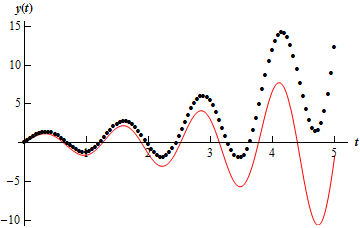
\includegraphics[width=\textwidth,height=\textheight,keepaspectratio]{p3-teaser.png}
\end{center}
\pagebreak

\section*{Introduction}

The goals of this practical are to:

\begin{itemize}
\item Modify the architecture to suit our evolving requirements
\item Implement a robust approach to timing
\item Develop a practical understanding of common numerical integration methods
\end{itemize}

You will continue working on and evolving the same project: ``02\_particles\_framework''.

\subsection*{Preparing demos for different scenarios}

As you have seen so far, and you will also see from the tasks that you have complete below, you will be asked to demonstrate a number of scenarios in your application: a particle bouncing in a cube, or several different particles, side-by-side, each with its own integration method, etc. There are several ways to accomplish this, and one of them is to copy-paste the code, make a new application and change the relevant code. \textbf{We will not be following this approach}, as it's very bad design, and violates the Don't Repeat Yourself (DRY) principle. There are several ways to accomplish this within a single application, and one of the simplest ones is the following:

\begin{itemize}
\item Use a variable to specify the scenario you are showing. This variable could be an integer, or better, an enum
\item Use input handling code to change the scenario according to the key you press
\item Make sure you initialise the scenario every time you switch to it: create particles, initialise their positions/velocities, etc.
\item Use an if/else if or switch statements in both the update and display functions, to only update/display things from the active scenario. Another similar approach would be to wrap related code in member functions of PhysicsEngine, such as Scenario1Initialise(), Scenario1Update() and Scenario1Draw() so that the bodies of PhysicsEngine::Init, PhysicsEngine::Update and PhysicsEngine::::Draw remain simple. 
\end{itemize}

\section*{Tasks}

\subsection*{Task 1: Particle bouncing in cube}

For this task, a particle needs to be bouncing inside a cubic room, as done in the last practical. Use gravity and aerodynamic drag as forces, and use impulses to implement collision response, as shown in the lecture materials. 

\textbf{Task: Implement a particle bouncing in a cubic room using gravity and aerodynamic drag forces}

\subsection*{Task 2: Integration methods}

As we have seen in the lecture, different integration methods are available and their performance is variable depending on the time step, but also on the type of simulation implemented. The purpose of this task is to give you an opportunity to witness the differences between simple integration techniques. You will do this by running the same simple simulation with three integrators: \textbf{Forward Euler}, \textbf{Semi-implicit} (or Symplectic) Euler, and \textbf{another one of your choice} (e.g. Verlet).

\textbf{Task: Implement a simulation of several bouncing particles, the only difference between each particle being the integration method used}

Here's information about how you should proceed:

\begin{itemize}
\item create 4 particles separated by a short distance on the x axis. In other words, the particles will be next to each other on your screen.
\item Translate each particle so that it sits a few units above the ground plane.
\item Keep the first one immobile (don't apply any force to it), it will act as a reference.
\item Apply gravity to the other 3 and use collision detection with the ground plane to ensure that the particles bounce on the plane without any loss of momentum. Give all particles an initial velocity of (0,0,0).
\item Run your simulation for various timestep values, say from 0.0005 to 0.1 and observe.
the differences of behaviours.
\end{itemize}

\subsection*{Task 3: Time step}

The performance of integration techniques is correlated to the size of the time step used. The smaller the timestep, the better integrators behave. The problem is that the timestep is not an independent variable of our simulation. It depends on the frequency at which we can perform our game loop, which depends on everything that goes on within the game loop, most notably physics computation and rendering. In our case, rendering will not be the problem, but physics computations will. 

The following page used to provide a good presentation of various approaches and their limitations: \url{https://gafferongames.com/post/fix_your_timestep}

Alternatively, read the following sections, in which I have copied the content almost verbatim.

Here's your task, keep it in mind as you read the rest of this section:

\textbf{Task: Implement the time step solution presented in the ``Free The Physics'' section of the above page}

You are welcome to implement the final solution presented in that article ``The final touch'', but you'll have to implement a concept of \emph{State}, which you are not expected to do at this stage.

\subsubsection*{Fixed delta time}

The simplest way to step forward is with fixed delta time, like 1/60th of a second:

\begin{minipage}{\linewidth}\begin{lstlisting}
double t = 0.0;
double dt = 1.0 / 60.0;
while ( !quit )
{
	integrate( state , t, dt );
	render( state );
	t += dt;
}
\end{lstlisting}\end{minipage}

In many ways this code is ideal. If you're lucky enough to have your delta time match the display refresh rate, and you can ensure that your update loop takes less than one frame worth of real time, then you already have the perfect solution for updating your physics simulation and you can stop reading this article. 

But in the real world you may not know the display refresh rate ahead of time. VSYNC could be turned off, or you could be running on a slow computer which cannot update and render your frame fast enough to present it at 60fps. 

In these cases your simulation will run faster or slower than you intended. 

\subsubsection*{Variable delta time}

Fixing this seems simple. Just measure how long the previous frame takes, then feed that value back in as the delta time for the next frame. This makes sense because of course, because if the computer is too slow to update at 60Hz and has to drop down to 30fps, you'll automatically pass in 1/30 as delta time. Same thing for a display refresh rate of 75Hz instead of 60Hz or even the case where VSYNC is turned off on a fast computer: 

\begin{minipage}{\linewidth}\begin{lstlisting}
double t = 0.0;
double currentTime = hires_time_in_seconds();
while ( !quit )
{
	double newTime = hires_time_in_seconds();
	double frameTime = newTime - currentTime;
	currentTime = newTime;
	integrate( state , t, frameTime );
	t += frameTime;
	render( state );
}
\end{lstlisting}\end{minipage}

But there is a huge problem with this approach which I will now explain. The problem is that the behavior of your physics simulation depends on the delta time you pass in. The effect could be subtle as your game having a slightly different ``feel'' depending on framerate or it could be as extreme as your spring simulation exploding to infinity, fast moving objects tunneling through walls and players falling through the floor!

One thing is for certain though and that is that it's utterly unrealistic to expect your simulation to correctly handle any delta time passed into it. To understand why, consider what would happen if you passed in 1/10th of a second as delta time? How about one second? 10 seconds? 100? Eventually you'll find a breaking point. 

\subsubsection*{Semi-fixed timestep}

It's much more realistic to say that your simulation is well behaved only if delta time is less than or equal to some maximum value. This is usually significantly easier in practice than attempting to make your simulation bulletproof at a wide range of delta time values. 

With this knowledge at hand, here's a simple trick to ensure that you never pass in a delta time greater than the maximum value, while still running at the correct speed on different machines:

\begin{minipage}{\linewidth}\begin{lstlisting}
double t = 0.0;
double dt = 1 / 60.0;
double currentTime = hires_time_in_seconds();
while ( !quit )
{
	double newTime = hires_time_in_seconds();
	double frameTime = newTime - currentTime;
	currentTime = newTime;
	while ( frameTime > 0.0 )
	{
		float deltaTime = min( frameTime , dt );
		integrate( state , t, deltaTime );
		frameTime -= deltaTime;
		t += deltaTime;
	}
	render( state );
}
\end{lstlisting}\end{minipage}

The benefit of this approach is that we now have an upper bound on delta time. It's never larger than this value because if it is we subdivide the timestep. The disadvantage is that we're now taking multiple steps per-display update including one additional step to consume any the remainder of frame time not divisible by dt. This is no problem if you are render bound, but if your simulation is the most expensive part of your frame you could run into the so called ``spiral of death''.

What is the spiral of death? It's what happens when your physics simulation can't keep up with the steps it's asked to take. For example, if your simulation is told: ``OK, please simulate X seconds worth of physics'' and if it takes Y seconds of real time to do so where Y $>$ X, then it doesn't take Einstein to realize that over time your simulation falls behind. It's called the spiral of death because being behind causes your update to simulate more steps to catch up, which causes you to fall further behind, which causes you to simulate more steps...

So how do we avoid this? In order to ensure a stable update I recommend leaving some headroom. You really need to ensure that it takes significantly less than X seconds of real time to update X seconds worth of physics simulation. If you can do this then your physics engine can ``catch up'' from any temporary spike by simulating more frames. Alternatively you can clamp at a maximum number of steps per frame and the simulation will appear to slow down under heavy load. Arguably this is better than spiraling to death, especially if the heavy load is just a temporary spike.

\subsubsection*{Free the physics (Task 3 required implementation)}

Now let's take it one step further. What if you want exact reproducibility from one run to the next given the same inputs? This comes in handy when trying to network your physics simulation using deterministic lockstep, but it's also generally a nice thing to know that your simulation behaves exactly the same from one run to the next without any potential for different behavior depending on the render framerate.

But you ask why is it necessary to have fully fixed delta time to do this? Surely the semi-fixed delta time with the small remainder step is "good enough"? And yes, you are right. It is good enough in most cases but it is not exactly the same due to to the limited precision of floating point arithmetic. 

What we want then is the best of both worlds: a fixed delta time value for the simulation plus the ability to render at different framerates. These two things seem completely at odds, and they are - unless we can find a way to decouple the simulation and rendering framerates. 

Here's how to do it. Advance the physics simulation ahead in fixed dt time steps while also making sure that it keeps up with the timer values coming from the renderer so that the simulation advances at the correct rate. For example, if the display framerate is 50fps and the simulation runs at 100fps then we need to take two physics steps every display update. Easy.

What if the display framerate is 200fps? Well in this case it we need to take half a physics step each display update, but we can't do that, we must advance with constant dt. So we take one physics step every two display updates. 

Even trickier, what if the display framerate is 60fps, but we want our simulation to run at 100fps? There is no easy multiple. What if VSYNC is disabled and the display frame rate fluctuates from frame to frame?

If you head just exploded don't worry, all that is needed to solve this is to change your point of view. Instead of thinking that you have a certain amount of frame time you must simulate before rendering, flip your viewpoint upside down and think of it like this: the renderer produces time and the simulation consumes it in discrete dt sized steps.

For example:

\begin{minipage}{\linewidth}\begin{lstlisting}
double t = 0.0;
const double dt = 0.01;
double currentTime = hires_time_in_seconds();
double accumulator = 0.0;
while ( !quit )
{
	double newTime = hires_time_in_seconds();
	double frameTime = newTime - currentTime;
	currentTime = newTime;
	accumulator += frameTime;
	while ( accumulator >= dt )
	{
		integrate( state , t, dt );
		accumulator -= dt;
		t += dt;
	}
	render( state );
}
\end{lstlisting}\end{minipage}

Notice that unlike the semi-fixed timestep we only ever integrate with steps sized dt so it follows that in the common case we have some unsimulated time left over at the end of each frame. This left over time is passed on to the next frame via the accumulator variable and is not thrown away.

\subsubsection*{The final touch}

But what do to with this remaining time? It seems incorrect doesn't it? To understand what is going on consider a situation where the display framerate is 60fps and the physics is running at 50fps. There is no nice multiple so the accumulator causes the simulation to alternate between mostly taking one and occasionally two physics steps per-frame when the remainders "accumulate" above dt.

Now consider that the majority of render frames will have some small remainder of frame time left in the accumulator that cannot be simulated because it is less than dt. This means we're displaying the state of the physics simulation at a time slightly different from the render time, causing a subtle but visually unpleasant stuttering of the physics simulation on the screen.

One solution to this problem is to interpolate between the previous and current physics state
based on how much time is left in the accumulator:

\begin{minipage}{\linewidth}\begin{lstlisting}
double t = 0.0;
double dt = 0.01;
double currentTime = hires_time_in_seconds();
double accumulator = 0.0;
State previous;
State current;
while ( !quit )
{
	double newTime = time();
	double frameTime = newTime - currentTime;
	if ( frameTime > 0.25 )
		frameTime = 0.25;
	currentTime = newTime;
	accumulator += frameTime;
	while ( accumulator >= dt )
	{
		previousState = currentState;
		integrate( currentState , t, dt );
		t += dt;
		accumulator -= dt;
	}
	const double alpha = accumulator / dt;
	State state = currentState * alpha +
	previousState * ( 1.0 - alpha );
	render( state );
}
\end{lstlisting}\end{minipage}

This looks complicated but here is a simple way to think about it. Any remainder in the accumulator is effectively a measure of just how much more time is required before another whole physics step can be taken. For example, a remainder of dt/2 means that we are currently halfway between the current physics step and the next. A remainder of dt*0.1 means that the update is 1/10th of the way between the current and the next state.

We can use this remainder value to get a blending factor between the previous and current physics state simply by dividing by dt. This gives an alpha value in the range [0,1] which is used to perform a linear interpolation between the two physics states to get the current state to render. This interpolation is easy to do for single values and for vector state values. You can even use it with full 3D rigid body dynamics if you store your orientation as a quaternion and use a spherical linear interpolation (slerp) to blend between the previous and current orientations.

\subsection*{Task 4: Blow dryer}

The final task will demand a little bit of creativity to turn a high-level description of the system's requirements into a working application. A particle bouncing around in a cubic room is not that exciting. What if one carved a hole in the middle of the floor, stuck a blow dryer through it and switched it on. This is what I'm asking you to do. The conical shape depicted in figure \ref{fig:blowdryer} represents the limits of the area in which the blow dryer has an effect. You can make the following assumptions about its behaviour:

\begin{itemize}
\item The force it generates is maximal at the bottom of the cone and zero at the top. The rate of decrease of the force field along the vertical axis is up to your experimentation. 
\item The force is maximal along the central vertical axis of the cone at any given height and decreases radially until it is zero at the edge of the cone. 
\item To begin with, you can assume that the force applied is always vertical (and directed upwards) at any position within the cone. If you implement the simulation this way, you will receive 3 out of 4 marks for this task. For full marks, you must model a force whose direction is vertical on the central axis and becomes parallel to the cone edge at the edges.
\end{itemize}

\textbf{Task: Simulate a ``blow dryer'' effect as described above and add it to the room.}

You'll need to experiment with the strength of the blow, the size of its area of influence until you achieve an interesting behaviour when a particle bounces around within the cube.

\begin{figure}[t]
\begin{center}
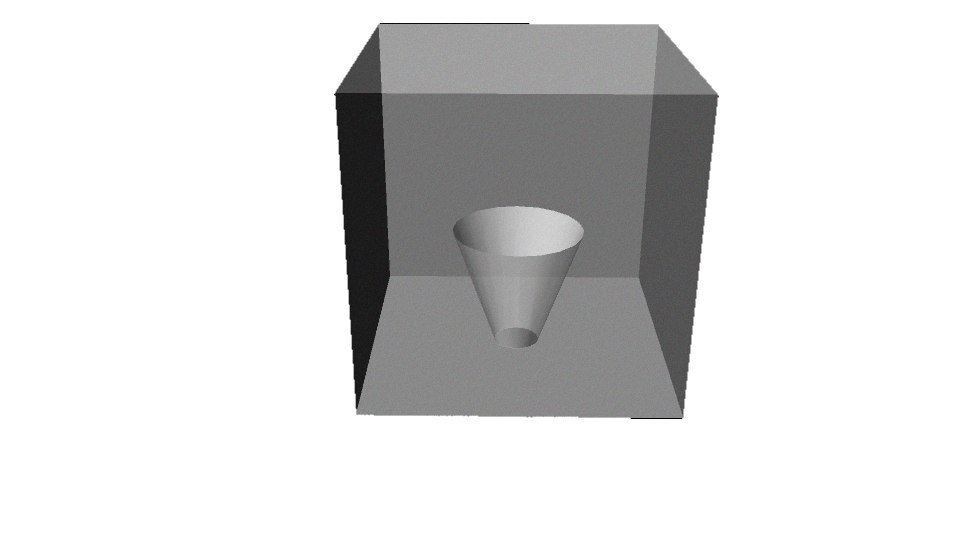
\includegraphics[width=\textwidth]{p3-blowdryer.png}
\caption{Example blow dryer shape and placement}
\label{fig:blowdryer}
\end{center}
\end{figure}

\section*{Deliverables}

This week's work (and a bit from last week) is assessed, so you need to submit evidence of completed tasks to gain credits.

\subsection*{Marking scheme}

Here's a summary of what you need to deliver, and the associated marks:

\begin{itemize}
\item \textbf{Particle bouncing within cube using this framework (Task 1): 4 marks}
\item \textbf{Implementation of Explicit and Symplectic Euler integration methods (Task 2): 4 marks} 
\item \textbf{Implementation of one additional integration method (Task 2): 4 marks}
\item \textbf{Implementation of timestep (Task 3): 4 marks}
\item \textbf{Addition of a blow dryer (Task 4): 4 marks} 
\end{itemize}

\subsection*{Submission details}

You must submit your work using the relevant Moodle assignment by the deadline specified on Moodle. Please submit, in a zip file:

\begin{itemize}
\item Your source code (/path-to-repository/code/02\_particles\_framework)
\item A working executable (/path-to-repository/code/build/bin/02\_particles\_framework.exe)
\item Instructions of how to use the program (key mappings, etc) as a text file
\end{itemize}

Marks will only be granted when a working application is demonstrated in the lab or via screen-sharing video.

\end{document}